\documentclass{../Vorlage/sebDenCls}
\usepackage{graphicx}
\usepackage{caption}
\usepackage{subcaption}
\usepackage{listings}
\usepackage{todo}
\usepackage{longtable}
\lstset{language=C++,basicstyle=\footnotesize}
\graphicspath{ {Bilder/Doku/} }

\setcounter{section}{3}
\setcounter{secnumdepth}{3}

\begin{document}
\fach{Echtzeitbildverarbeitung}
\nr{3}
\abgabe{04.07.2017}
\semester{SoSe17}
\blatt{Udo Frese}{Lukas Bertram}{(lbertram@uni-bremen.de)}{Sebastian Bliefert}{(bliefert@uni-bremen.de)}{Johannes Hochbein}{(hochbein@uni-bremen.de)}{Pascal Pieper}{(ppieper@uni-bremen.de)}

\section{Die Idee}
Es wurde ein eigenes Framework geschrieben, um die verschiedenen Anwendungsgebiete effizient abdecken zu können. In der Datei \texttt{licenseRecognizer.cpp} ist die Hauptroutine implementiert.
Hier wird entschieden, ob die Bildverarbeitung auf statische Bilddateien oder auf kontinuierliche Bildern einer angeschlossenen Kamera angewandt werden soll.
Die Funktionen \texttt{imagePath()} und \texttt{camPath()} sind jeweils dazu da, die verschiedenen Quellen einzulesen und durch \texttt{pipelineDetect()} analysieren zu lassen. Die Bilderkennung ist in logische Abschnitte unterteilt, die jeweils in der Funktion \texttt{pipelineDetect()} angewandt werden.\\
Zuerst wird das Bild durch \texttt{preprocessing()} vorverarbeitet (siehe Kapitel \ref{prepro}). Dieses Bild wird dann durch \texttt{findPlates()} (Kapitel \ref{findpl}) analysiert, und Eckpunkte des erkannten Nummernschildes in das \texttt{deWarp()} (Kapitel \ref{dewarp}) geliefert. Dieses beschneidet und entzerrt das Originalbild zu einem Ausschnitt. Daraufhin wird es durch ein klassisches \texttt{dilate()} und \texttt{erode()} von kleineren Flecken befreit. In Funktion \texttt{plateRecog()} wird dieser Ausschnitt dann der Texterkennung \texttt{customOCR::ocr()} übergeben, welches alle erkannten Wörter bzw. Buchstaben zurückliefert (siehe Kapitel \ref{lookupPlate}), und anschließend werden die gefundenen Buchstaben mit bekannten Nummernschildern verglichen. Ist ein bekanntes dabei, wird die entsprechende ID zurückgegeben, und ggfs. eine zugeordnete Funktion ausgeführt (bspw. Tor öffnen).

\subsection{Anmerkung}
\textit{Um die beigefügten Programmdateien ausführen oder kompilieren zu können, muss die OCR-Bibliothek tesseract zunächst installiert werden. Eine Anleitung dazu findet sich in ./Readme.txt.
}

\subsection{cropImage}
Diese ursprünglich geplante Methode wird nicht mehr benötigt. Die Bilder sind im Urzustand nicht so groß wie befürchtet. Ein weiterer Vorteil ist, dass der auswertbare Bildbereich nicht von Anfang an beschnitten wird. Dies gibt später mehr Spielraum für die Positionierung der Fahrzeuge.
\subsection{preprocessing}
\label{prepro}
Zu Beginn der Bildverarbeitung wird die Funktion \texttt{preprocessing()} aufgerufen, um eine Anpassung der Farbinformationen und des Kontrastes vorzunehmen, um für die Kennzeichenerkennung irrelevante Informationen so gut wie möglich aus dem Bild zu entfernen.
Insbesondere werden alle Grauwerte, die gewöhnlich nicht zum Nummernschild gehören, durch die Verarbeitung ins Schwarze gezogen, während die helleren Bildbereiche weiter erhellt werden. Dadurch wird das Nummernschild so gut wie möglich isoliert. Die Parameter für Kontrast-, Gamma-  und Helligkeitsanpassung wurden anhand der vorhandenen Testbilder empirisch ermittelt und müssen dementsprechend bei Verwendung des Systems in anderem Aufbau an die Verhältnisse angepasst werden. Der Algorithmus ist angelehnt an die in \cite{gimp17} vorgestellte Logik zur Farbanpassung.\\

\begin{figure}[htp]
	\centering 	
	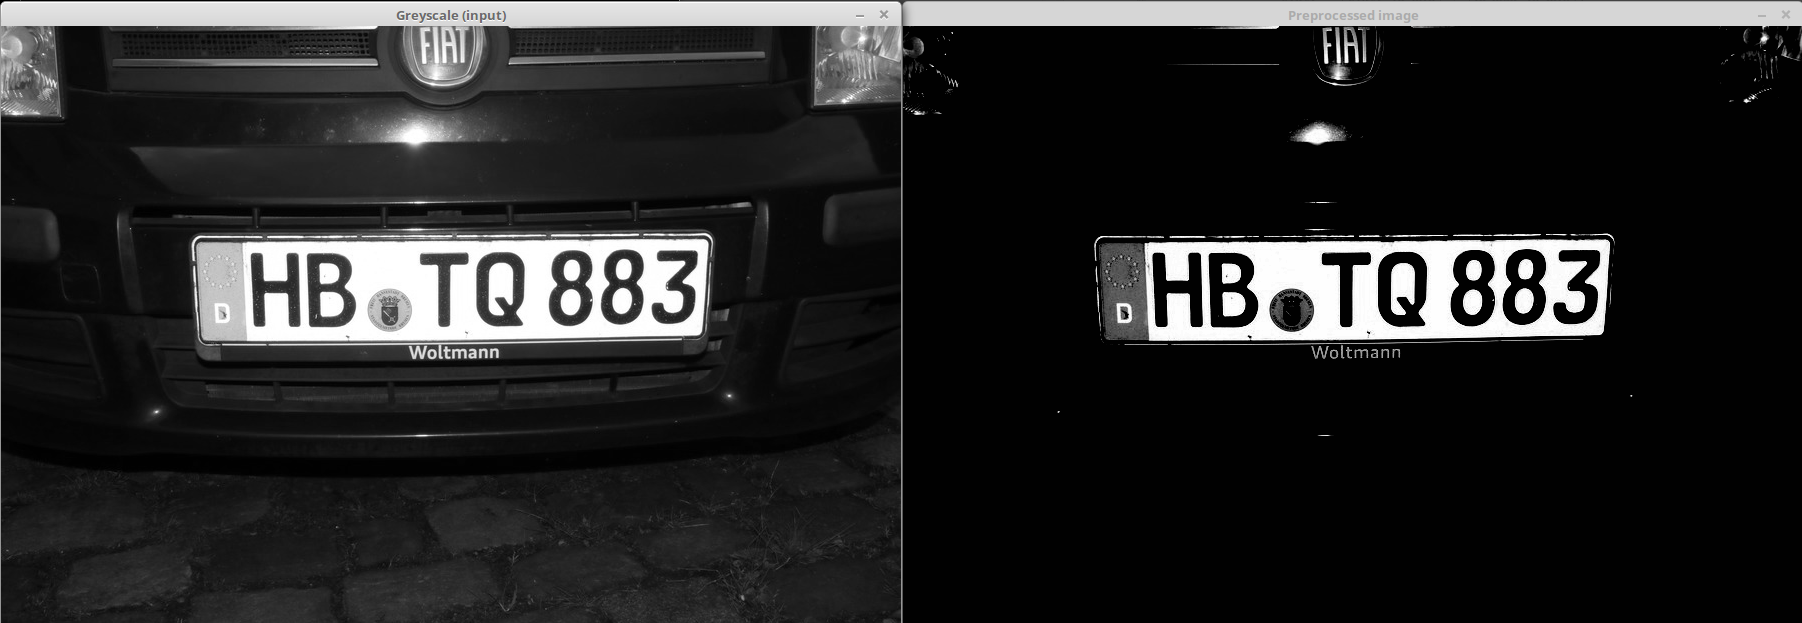
\includegraphics[width=.9\textwidth]{beispiel_preprocessing} 
	\caption{Eingabebild (links), Ausgabebild (rechts) \label{beispiel_preprocessing}}
\end{figure}

Die Funktion \texttt{preprocessing()} sieht folgendermaßen aus:\\
\lstinputlisting[firstnumber=30, firstline=30, lastline=82]{coreFunctions.cpp}


\subsection{detectLines}
Die ursprünglich geplante Funktion \texttt{findLines()} wurde während der Implementationsphase in die Funktion \texttt{findPlates()} übernommen. 

\subsection{findPlates}
\label{findpl}

Nach erfolgter Vorverarbeitung durch \texttt{preprocessing()} erfolgt die Extraktion der Kennzeichenkontur in \texttt{findPlates()}. Dazu werden zunächst die Kanten im Bild durch die Verwendung des Canny-Algorithmus gefunden und mithilfe von \texttt{findContours()} in relevante Konturen umgewandelt. Zu jeder gefundenen Kontur wird die konvexe Hülle berechnet, um zusammenhängende Konturen zu erhalten und etwaige Unterbrechungen und Einschlüsse zu eliminieren. Anschließend erfolgt eine Vereinfachung jeder konvexen Hülle mithilfe des \texttt{approxPolyDP()} Algorithmus, welcher die Anzahl der Eckpunkte des die Hülle darstellenden Polygons mithilfe von Approximation reduziert (genauere Informationen zum genutzen Algorithmus in \cite{opCV14}). Die vereinfachten Konturen werden im Anschluss nach der Größe ihrer Fläche verglichen, um die größte Kontur zu finden, welche grundsätzlich für das Nummernschild gehalten wird. Falls diese Kontur nach der ersten Approximation noch nicht über exakt vier Eckpunkte verfügt, wird sie zyklisch weiter vereinfacht, bis dieses Kriterium erfüllt ist. Abschließend werden die so gewonnenen Eckpunkte in die für die weitere Verarbeitung richtige Reihenfolge gebracht und ausgegeben.

Die Funktion \texttt{findPlates()} sieht folgendermaßen aus:\\

\lstinputlisting[firstnumber=84, firstline=84, lastline=223]{coreFunctions.cpp}

\begin{figure}[h]
	\centering 	
	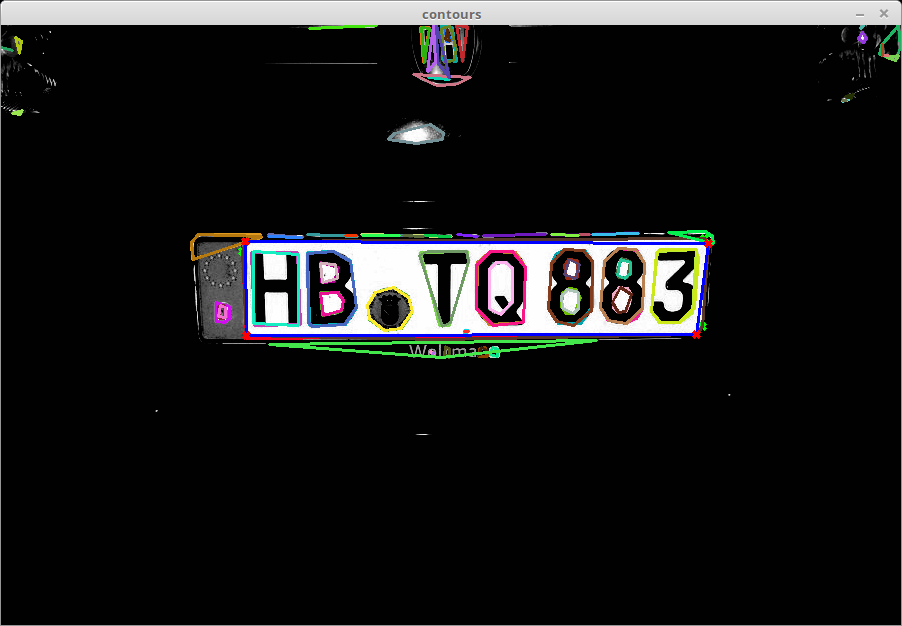
\includegraphics[width=.75\textwidth]{beispiel_kontur} 
	\caption{gefundene Konturen nach der ersten Approximation (bunte Konturen) und endgültige Kontur mit 4 Eckpunkten (blaue Kontur mit rot markierten Eckpunkten) \label{beipsiel_kontur}}
\end{figure}


\subsection{cropPlate}
\label{croppl}
Diese Funktion wurde an den Anfang von \texttt{deWarp()} ausgelagert und sieht folgendermaßen aus:\\
\lstinputlisting[firstnumber=224, firstline=224, lastline=310]{coreFunctions.cpp}
Zuerst werden Fehlerfälle aussortiert und zwei Debug-Fenster initialisiert. Ab Zeile 240 beginnt das eigentliche Croppen. \\
Zuerst werden die minimalen x- und y-Werte ermittelt und dann aus diesen ein Rechteck von den jeweiligen Minima bis Maxima aufgespannt. Dieses wird dann in Zeile 251 zum Croppen des Bildes genutzt.\\
Am Ende wird im debugmodus noch das Ergebnis angezeigt.
\subsection{deWarp}
\label{dewarp}
Erster Teil des Quellcodes siehe Kapitel \ref{croppl} cropPlate.
\lstinputlisting[firstnumber=253, firstline=253, lastline=281]{coreFunctions.cpp}
Im zweiten Teil der deWarp-Funktion wird erst das Nummernschildformat abgeschätzt. Dazu wird ein Aspect-Ratio-Threshold benutzt, der sich aus der Aspect-Ratio des zweireihigen Nummernschildes ableitet. Anhand dieses Thresholds wird entschieden, ob es sich vermutlich um ein ein- oder zweireihiges Nummernschild handelt.\\
Nun folgt das eigentliche Warpen. Dazu werden als erstes die Destination-Koordinaten anhand der zuvor ermittelten Nummernschildform festgelegt und die Source-Koordinaten auf das neue (gecroppte) Bild umgerechnet. Dann übernimmt openCV die eigentliche Berechnung der Transformationsmatrix und das Warpen selbst.\\
Schlussendlich wird noch als Hilfestellung für die Texterkennung ein weißer Rahmen um das verarbeitete Nummernschild gezogen und das Ergebnis zurückgegeben.

\subsection{getText}
Implementiert in Klasse \texttt{CustomOCR} und \texttt{LexiconOCR}.
Die Klasse \texttt{LexiconOCR} war ein erster Versuch, einzelne Wörter zu erkennen. Dies hat nicht zufriedenstellend funktioniert, da pro Bild nur ein Wort erwartet wurde. Daher wird hier auch keine Dokumentation dazu erstellt.
\texttt{CustomOCR} ist eine Klasse, die an das Beispiel von OpenCV's Texterkennungsbeispiel angelehnt ist. Von dort sind auch die \textit{ER-Groupings}, die das trainierte Neuronale Netz für die Buchstabensegmentierung und -Erkennung beinhalten. Die \texttt{CustomOCR::ocr()} Funktion wurde weiterhin effizienter gestaltet, sowie im Vorhinein bekannte Elemente wie die \textit{ER-Filter} in den Konstruktor umgelagert, um die Ausführzeit weiter zu verringern.

\lstinputlisting[firstnumber=19,firstline=19,lastline=140]{ocrBackend.cpp}

\subsection{lookupPlate}
\label{lookupPlate}
Diese Funktion sucht nach definierten Kennzeichen in erkanntem Text. Sie ist nicht besonders effizient implementiert, funktioniert aber schnell genug.\\
Jeder gefundene Textabsatz wird überprüft, ob von einem der definierten Nummernschilder alle Elemente enthalten sind. Wenn alle vorhanden sind, ist das Kennzeichen offiziell erkannt. Da die Texterkennung mit einer anderen Schriftart angelernt wurde, und die Kennzeichenschrift in einigen Buchstaben sehr eigen ist (um die Fälschung zu erschweren), sind Buchstaben wie \texttt{Y} und \texttt{V} sowie \texttt{I}, \texttt{1} und \texttt{l} häufig verwechselt. Da es sich bei dem System nicht um eine sicherheitsrelevante Anwendung handelt, wurden für die Tests auch die verwandten Buchstaben erlaubt (siehe Datei \texttt{knownPlates.hpp}).
\lstinputlisting[firstnumber=309,firstline=309,lastline=353]{coreFunctions.cpp}

\section{Ergebnisse}
\subsection{Testbedingungen}
Für den Test unserer Nummernschilderkennung haben wir verschiedene „Fälle“ generiert. Jeder Fall soll hierbei ein Beispiel eines sich dem Tor nähernden Fahrzeugs sein. So zeigt der Fall „A“ das Fahrzeug HB TQ-883 welches sich ohne Winkel der Kamera nähert. Die verschiedenen Bilder sollen hierbei den zeitlichen Verlauf des Heranfahrens darstellen. Es würde ausreichen, wenn auf einem der Bilder das Kennzeichen erkannt wird, da somit das Tor geöffnet werden würde, während sich das Fahrzeug nähert. Da Fahrzeuge nicht immer den exakt gleichen Weg fahren, haben wir weitere Fälle erstellt, bei denen das Fahrzeug jeweils einen Winkel zur Kamera hat, sodass diese nicht frontal auf das Kennzeichen schaut. Auch hier nähert sich das Fahrzeug mit jedem Bild wieder an die Kamera an (mit gleichbleibenden Winkel). Für jede Winkeländerung wurde ein neuer Fall erstellt,
sodass die Fälle A-E alle zum gleichen Fahrzeug gehören aber unterschiedliche Anfahrten darstellen.

Die von uns betrachteten Winkel sind teilweise sehr groß und überschreiten die von uns erwarteten Winkel die innerhalb einer Auffahrt gemacht werden können erheblich. Dies soll sicherstellen, dass die Erkennung auch unter extremen Bedingungen zufriedenstellend funktioniert.

Die Fälle F-J wurden für das Fahrzeug HB XY-84 erstellt. Hierbei gab es die weitere Schwierigkeit, dass die weiße Kunststoffoberfläche des Fahrzeuges das Licht der Kamera ähnlich gut reflektiert wie das Kennzeichen, sodass eine Abgrenzung des Kennzeichens schwieriger als bei den vorherigen Fällen ist.

Die Fälle K-O gehören zum Fahrzeug HB TI-326. Hier besteht die zusätzliche Schwierigkeit darin, dass das Fahrzeug durch eine längere Autobahnfahrt ein mit Insekten verschmutztes Kennzeichen hat.

Ein Problem bei der Erkennung mit der "tesseract" Bibliothek war, dass die Schriftart von Kennzeichen (FE-Schrift) dafür entwickelt wurde, dass diese nicht verfälscht werden können (Beispielsweise 3 zu 8). Diese sehr spezielle Schriftart wird deshalb allerdings standardmäßig von der Bibliothek nicht besonders gut erkannt. Da ein Anlernen der Schriftart sehr zeitintensiv ist, haben wir uns für unseren Test darauf beschränkt, in der Kennzeichenüberprüfung ähnliche Buchstaben, z.B. V anstelle von Y, gleichzustellen.\\

\textit{\textbf{Anmerkung}: Aufgrund der Größenbeschränkung für Uploads sind in der aktuellen Abgabe nicht alle Bilder für alle genannten Testfälle enthalten, können aber auf Nachfrage gerne zur Verfügung gestellt werden.}

\subsection{Ergebnis}
Es hat sich gezeigt, dass in jedem Anfahrtsszenario mindestens ein Bild erkannt wurde. Bei den einfachen Fällen A-E wurde in der Regel sogar auf fast allen Bilder das Kennzeichen richtig erkannt.
Debugausgaben einzelner erkannten Kennzeichen sind exemplarisch in Abb. \ref{beispiel} und Abb. \ref{beispiel2} dargestellt.

\begin{figure}[htp]
	\centering 	
	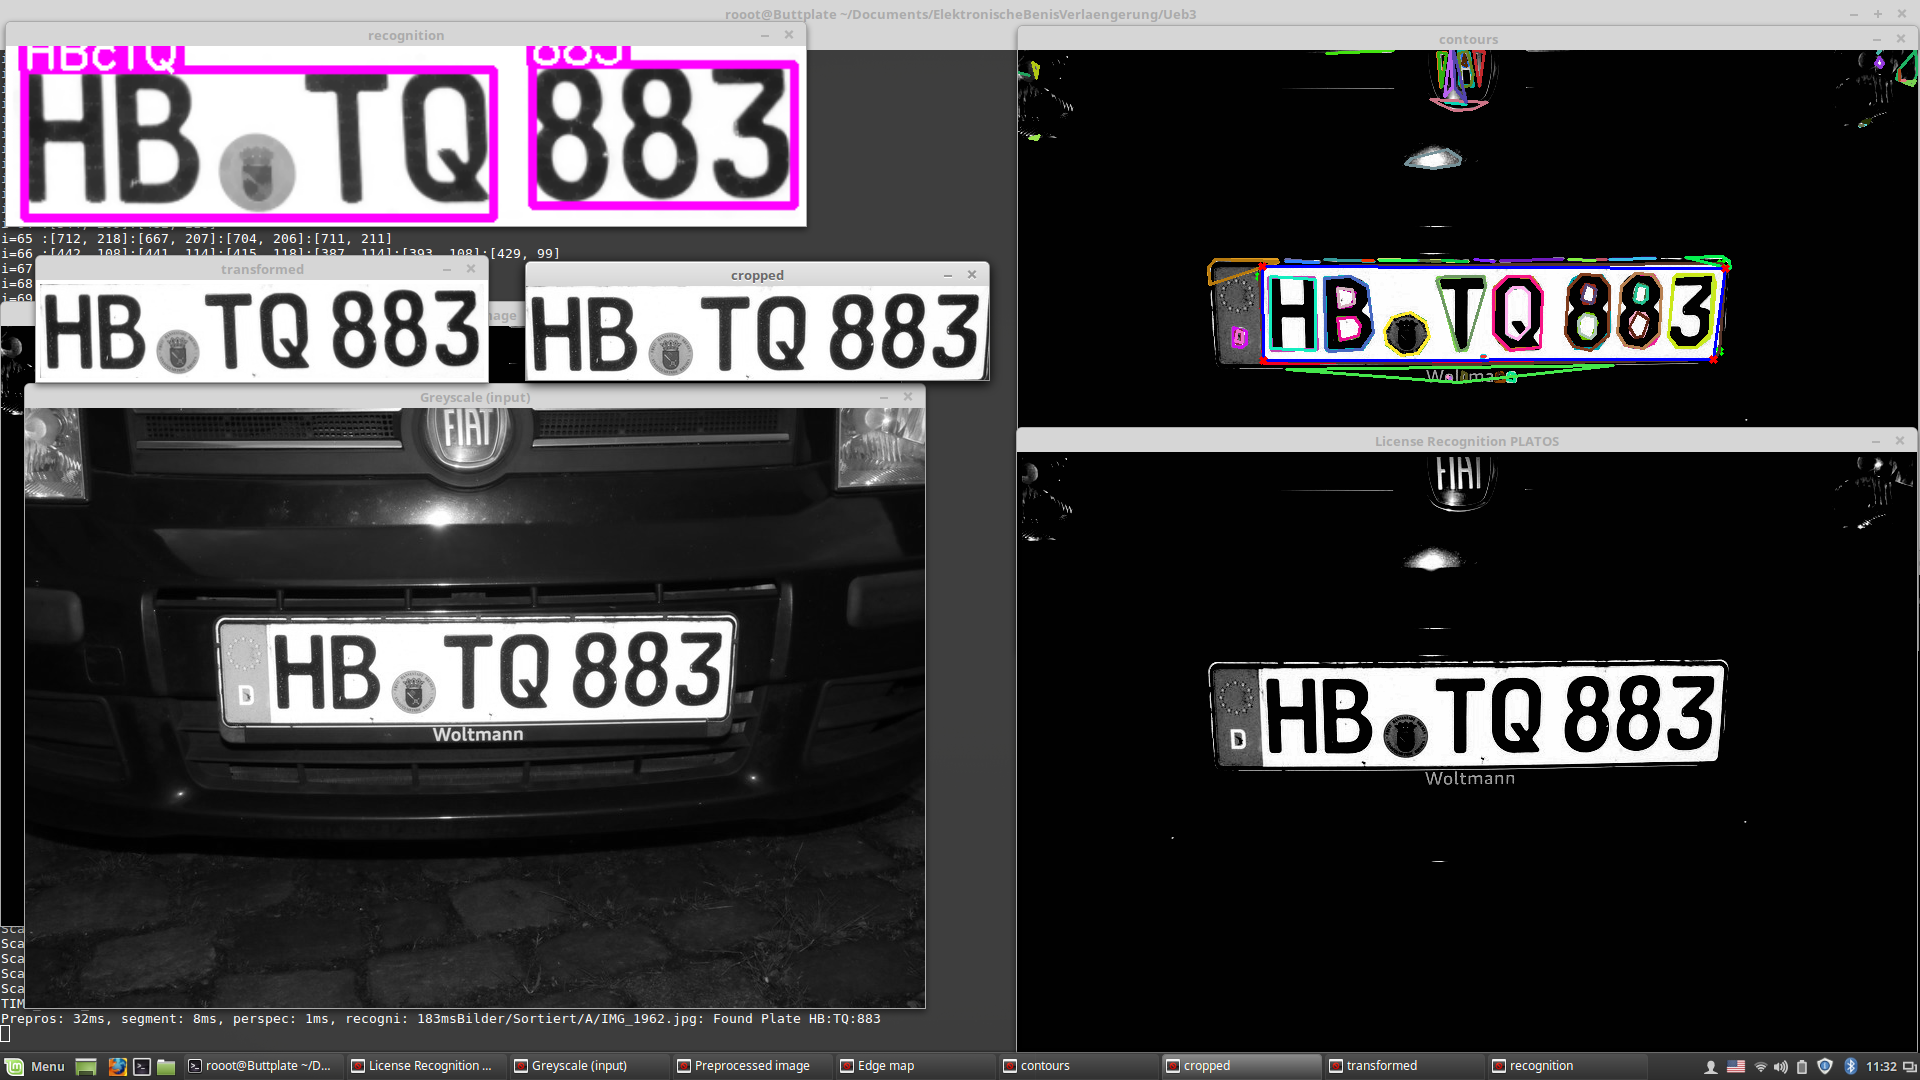
\includegraphics[width=.9\textwidth]{Funktioniert_1962.png} 
	\caption{Erkennung Beispielbild: Abstand $d=1m$, Winkel $\alpha = 0^\circ$ \label{beispiel}}
\end{figure}

\begin{figure}[htp]
	\centering 	
	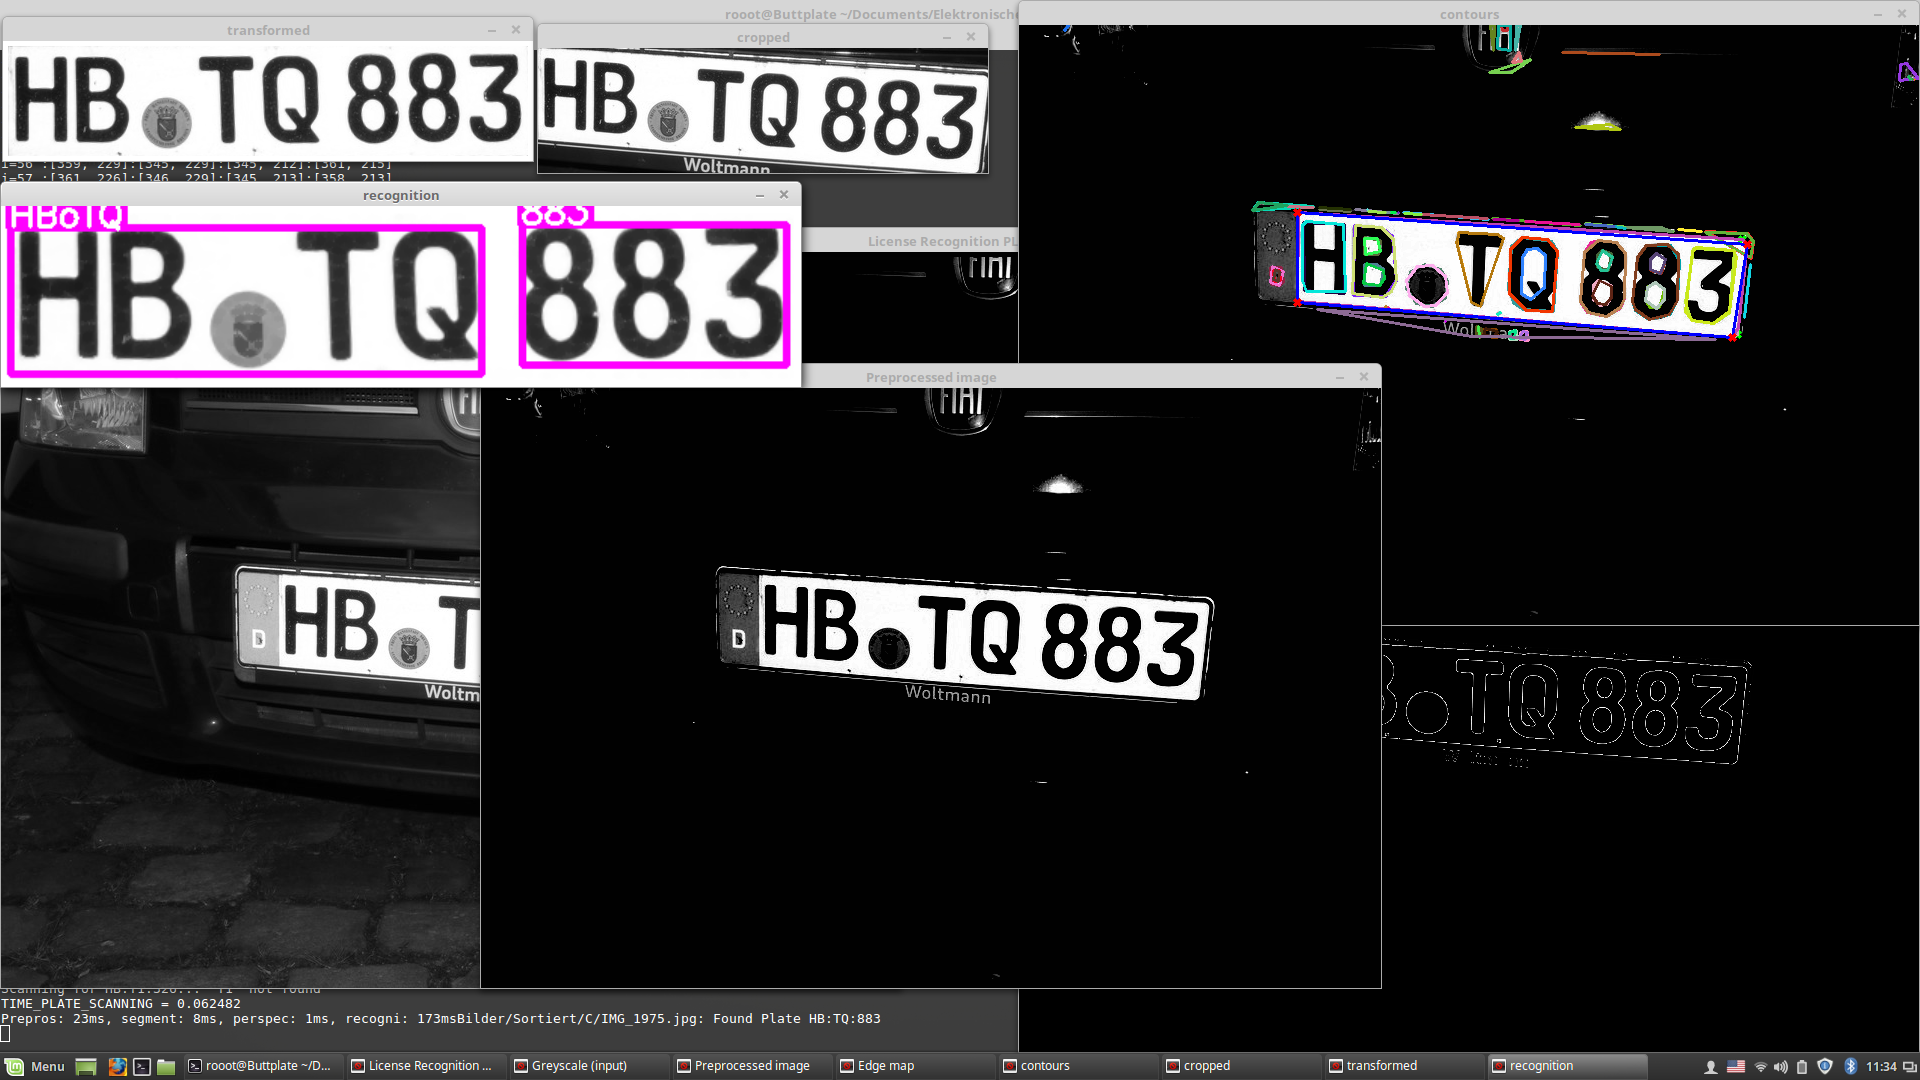
\includegraphics[width=.9\textwidth]{Funktioniert_1975.png} 
	\caption{Erkennung Beispielbild: Abstand $d=1m$, Winkel $\alpha = 20^\circ$ \label{beispiel2}}
\end{figure}


\subsection{Bewertung}
Es hat sich gezeigt, dass die von uns erstellte Kennzeichenerkennung bereits sehr gute Ergebnisse liefert, insbesondere, da in der Realität einer späteren Anwendung ein Videostream von dem heranfahrenden Fahrzeug vorhanden ist, sodass bei einer Geschwindigkeit von 10-30 Bildern/Sekunde eine deutlich größere Anzahl von Bildern zur Verfügung steht. Außerdem konnte bei Tests mit einer Webcam bereits beobachtet werden, dass falsch erkannte Buchstaben häufig „Springen“ sodass diese temporär auch richtig erkannt wurden. 

Dies zeigt allerdings auch, dass dieses System nicht für sicherheitsrelevante Zugänge geeignet ist, sondern rein der Erhöhung des Komforts dienen sollte. Eine Öffnung durch Fehlerkennung oder Manipulation durch einen Ausdruck eines Kennzeichens können nicht ausgeschlossen werden.
\section{Ausblick}
Als Ausblick für eine zukünftige Verbesserung möchten wir die Möglichkeit nennen, die Schriftart der Kennzeichen anzulernen, sodass Fehlerkennungen deutlich seltener vorkommen sollten.
Eine Weitere Verbesserung wäre es, eine Kamera mit Infrarotfilter einzusetzen und die Einfahrt mit Infrarotstrahlern zu beleuchten, dies hätte den Effekt, dass auf den Bildern Hauptsächlich nur noch das Kennzeichen zu sehen ist, da diese infrarotes Licht besonders gut reflektieren.

\section{Zeitverbrauch}
Wir haben an dem Projekt ungefähr 120 Mannstunden investiert.

\begin{thebibliography}{9}
	
	\bibitem{opCV14}
	OpenCV Documentation,
	\emph{Structural analysis and shpe descriptors - approxPolyDP(...)},
	\url{http://docs.opencv.org/2.4/modules/imgproc/doc/structural_analysis_and_shape_descriptors.html#approxpolydp},
	abgerufen am 01.07.2017, 17:30 Uhr.
	
	\bibitem{gimp17}
	GIMP Documentation,
	\emph{Chapter 4. Point operations},
	\url{https://pippin.gimp.org/image-processing/chap_point.html},
	abgerufen am 01.07.2017, 18:00 Uhr.
\end{thebibliography}

\end{document}


